\chapter{}
\label{app:A}

Something about the previous scattering results...  most likely due to L1 cache being removed in Kepler (L1 is local, not cached, Fermi had a L1)

\begin{figure}[h!] 
  \centering
    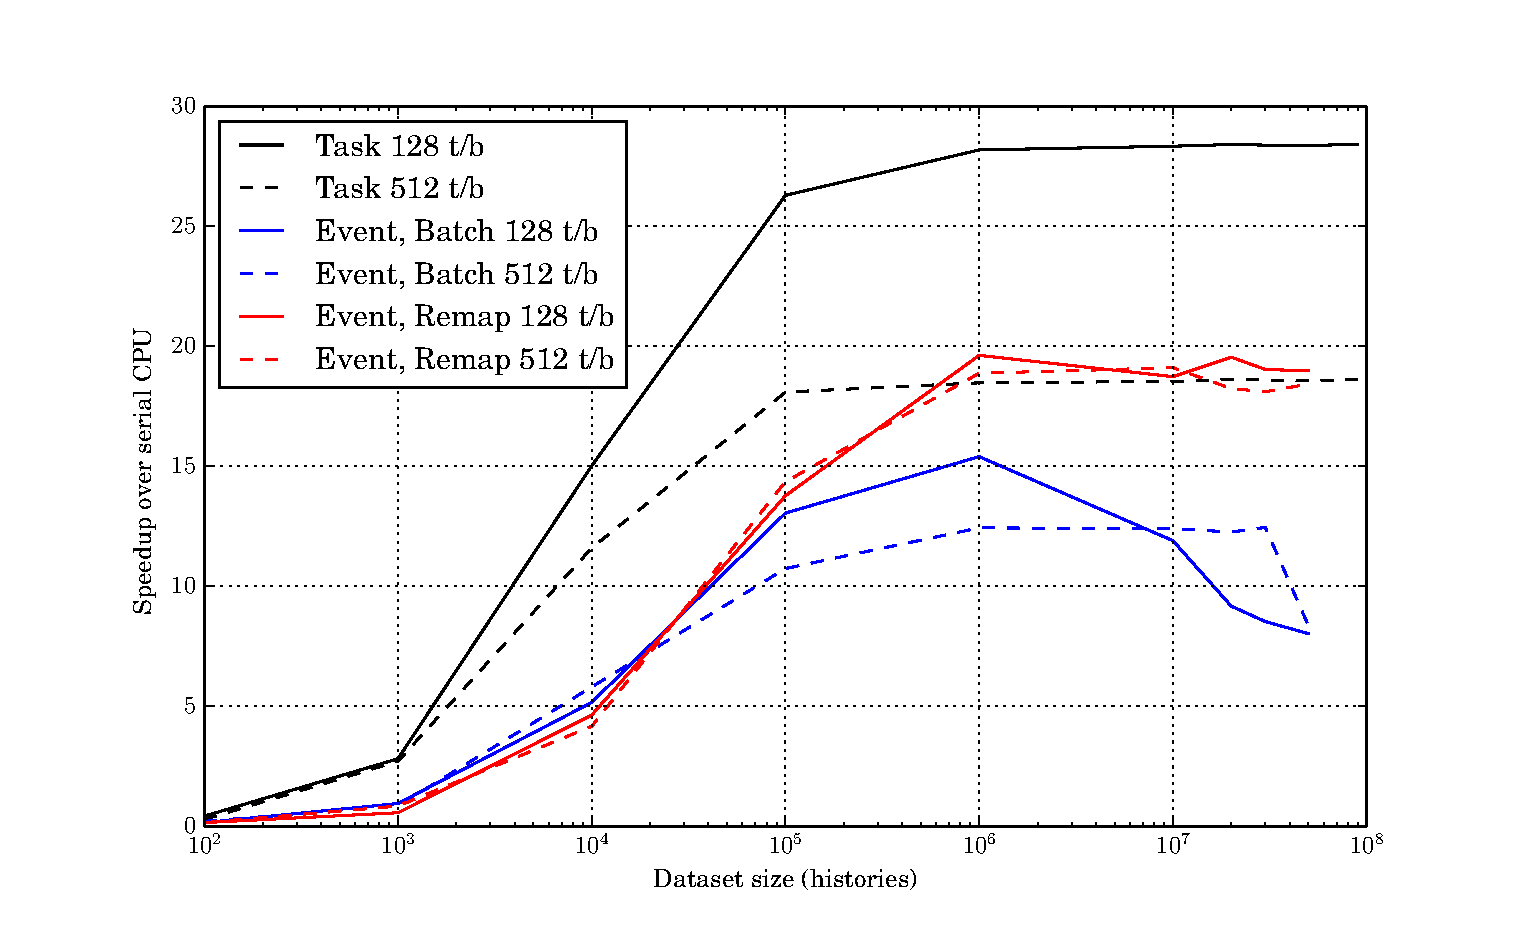
\includegraphics[width=0.8\textwidth]{graphics/prelim_speedup_old.eps}
     \caption{Speedup factors of the GPU implementations over the CPU implementation on a Tesla C2075. \label{prelim_speedup_old} }
\end{figure}

Figure \ref{prelim_speedup_old} shows the speedup factors, $F_s=t_\mathrm{CPU}/t_\mathrm{GPU}$, of the GPU implementations discussed in Section \ref{sec:prelim}.  This benchmark was run on the same server with a 8-core AMD Opteron 6128 CPU clocked at 2.0GHz, but on a Tesla C2075 card.  The task-parallel implementation performs best, with a maximum speedup of around 29x.  The remapping implementation has the next best performance, with about a 20x speedup over the CPU. The batched implementation's performance departs from the remapping implementation at $10^5$ particles and even starts to deteriorate between $10^6$ and $10^7$ particles.  This is due to the transport having to be done in batches at this point due to the maximum block number of 65,536.

\begin{figure}[h!] 
  \centering
    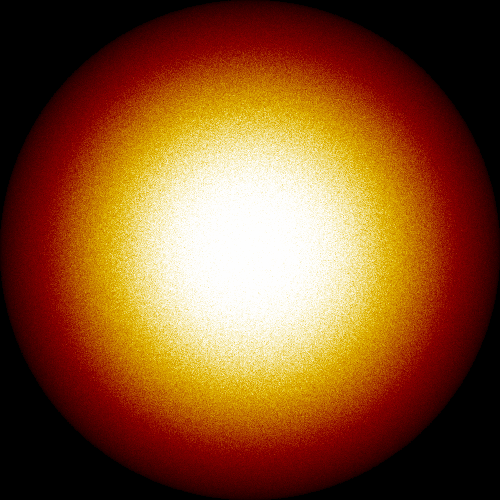
\includegraphics[width=0.5\textwidth]{graphics/finalresults/serpent-benchmark-6/godiva_mesh1.png}
     \caption{Fission source (orange/white) and thermal flux (blue/white) from Serpent 2.1.18 of a ``Jezebel'' bare Pu-239 sphere. \label{serp_godiva_mesh} }
\end{figure}

\begin{figure}[h!] 
  \centering
    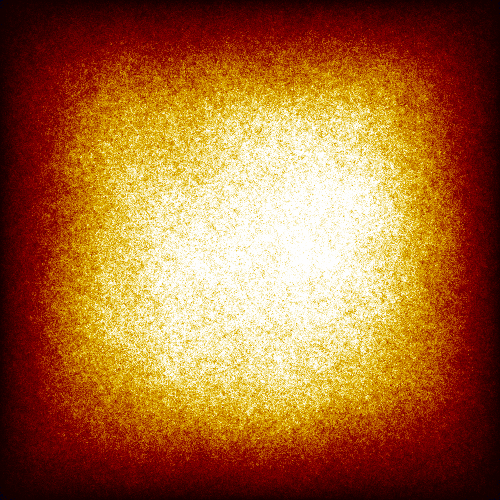
\includegraphics[width=0.5\textwidth]{graphics/finalresults/serpent-benchmark-6/homfuel_mesh1.png}
     \caption{Fission source (orange/white) and thermal flux (blue/white) from Serpent 2.1.18 of a homogenized block of UO$_2$ and water. \label{serp_homfuel_mesh} }
\end{figure}

\begin{figure}[h!] 
  \centering
    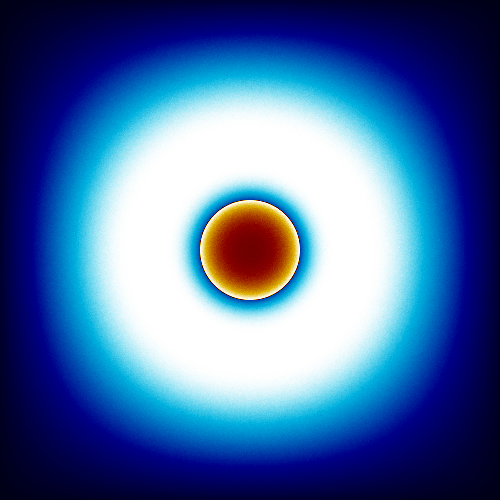
\includegraphics[width=0.5\textwidth]{graphics/finalresults/serpent-benchmark-6/pincell_mesh1.png}
     \caption{Fission source (orange/white) and thermal flux (blue/white) from Serpent 2.1.18 of a single UO$_2$ pin surrounded by a block of water  \label{serp_pincell_mesh} }
\end{figure}

\begin{figure}[h!] 
  \centering
    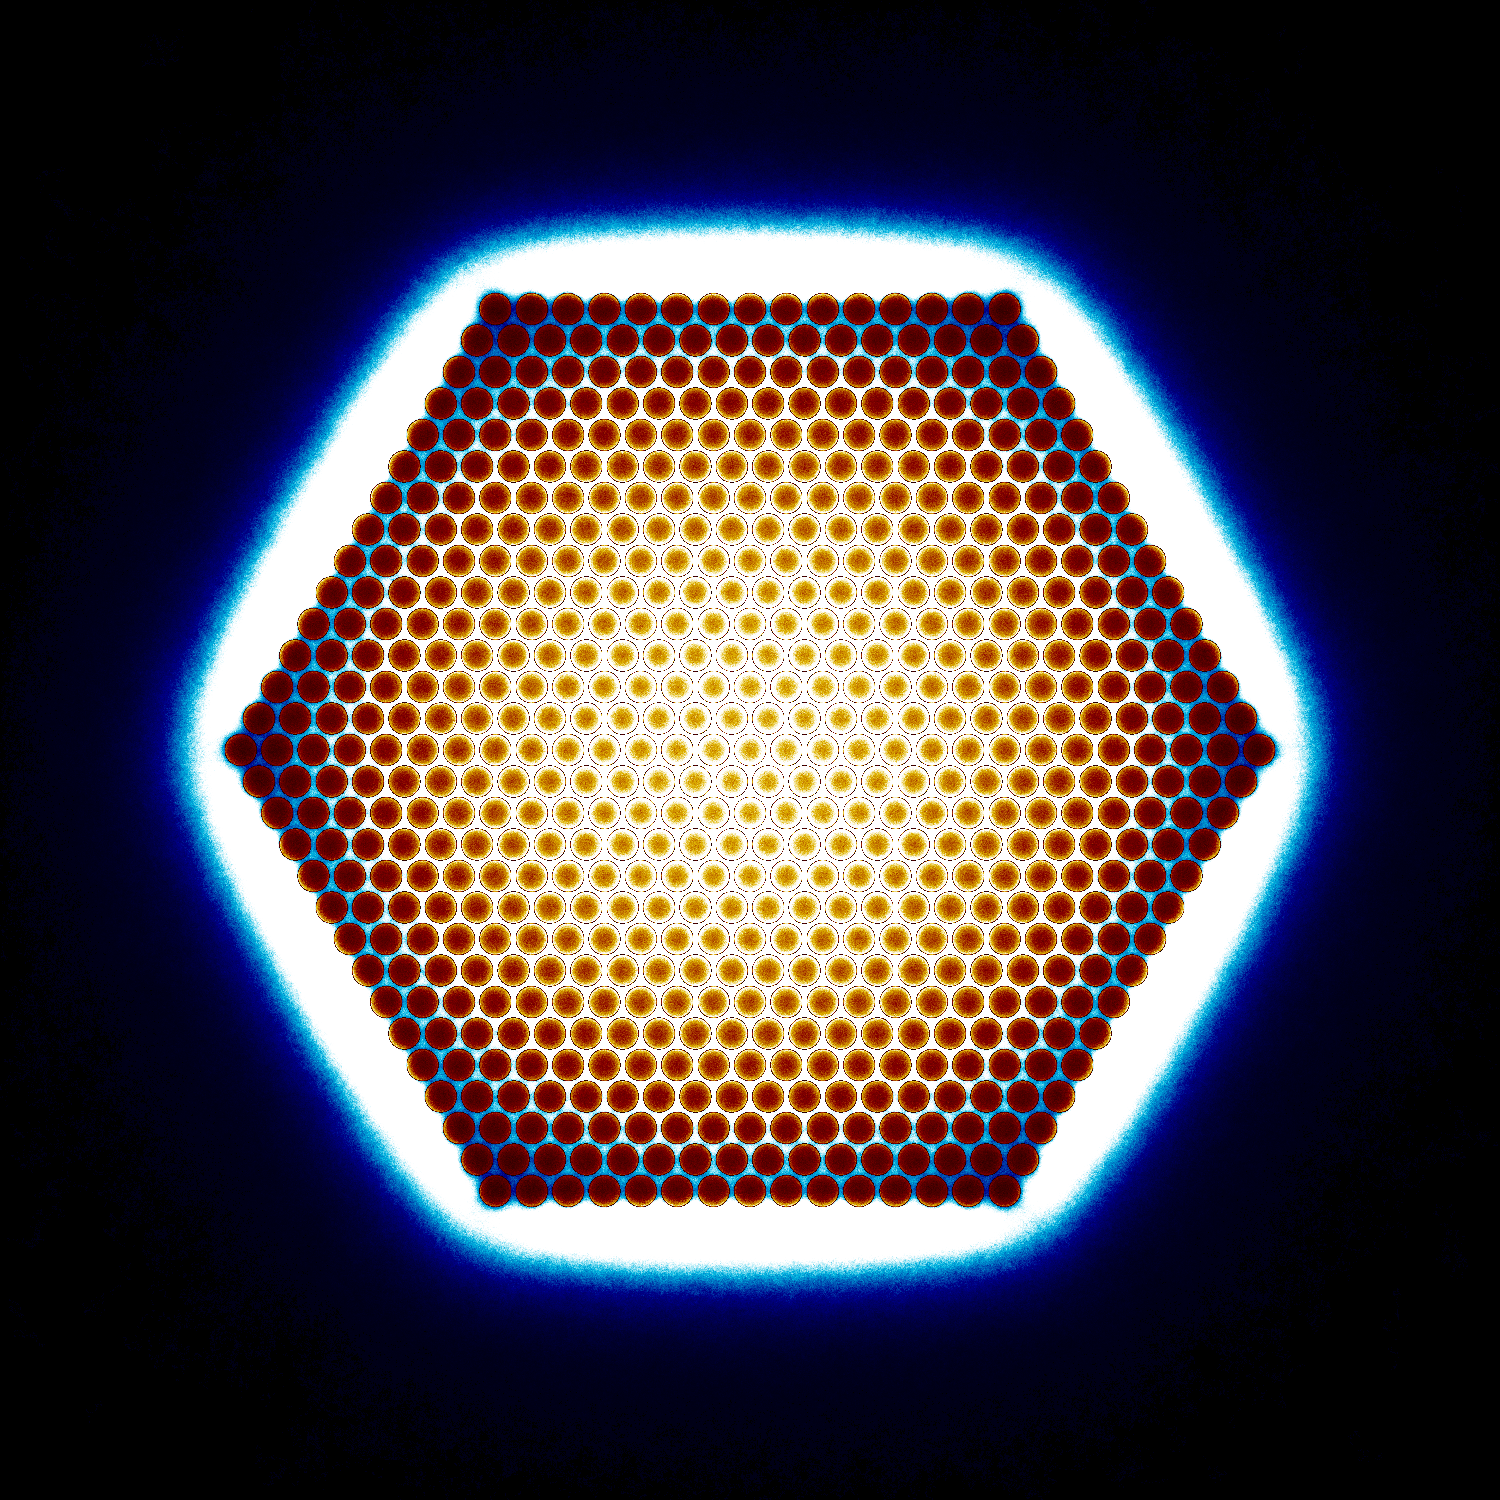
\includegraphics[width=0.5\textwidth]{graphics/finalresults/serpent-benchmark-6/assembly_mesh1.png}
     \caption{Fission source (orange/white) and thermal flux (blue/white) from Serpent 2.1.18 of a 15-sided hexagonal array of UO$_2$ pins in water. \label{serp_assembly_mesh} }
\end{figure}
